%\section{Introduction}
%\begin{itemize}
%	\item Bias -> fairness metric 
%	\item Fairness influence function (FIF)
%	\item Example
%	\item Contribution (1) framework (2) algorithm (3) experimental validation
%	\item Related works.
%	\item Notation paragraph
%\end{itemize}
The last decades have witnessed a significant progress in machine learning with applications in high-stake decision making, such as college admission~\cite{martinez2021using}, recidivism prediction~\cite{tollenaar2013method}, job applications~\cite{ajunwa2016hiring} etc. In such applications, the deployed machine learning classifier often demonstrate bias towards certain demographic groups involved in the data~\cite{dwork2012fairness}. For example, a classifier deciding the eligibility of college admission may offer more admission to White-male candidates than to Black-female candidates\textemdash possibly because of the historical bias in the admission data, or the accuracy-centric learning objective of the classifier, or a combination of both~\cite{berk2019accuracy,landy1978correlates,zliobaite2015relation}. Following such phenomena, multiple fairness metrics, such as \textit{statistical parity}, \textit{equalized odds}, \textit{predictive parity} etc, have been proposed to quantify the bias of the classifier on a dataset. For example, if the classifier in college admission demonstrates a {statistical parity} of $ 0.6 $, it means that White-male candidates are offered admission $ 60\% $ more than Black-female candidates~\cite{besse2021survey,feldman2015certifying,garg2020fairness}.

Although fairness metrics globally quantify bias, they cannot detect or explain the sources of bias~\cite{begley2020explainability,lundberg2020explaining,pan2021explaining}. In order to identify the sources of bias and also the effect of affirmative/punitive actions to alleviate/deteriorate bias, it is important to understand \textit{which factors contribute how much to the bias of a classifier on a dataset}. To this end, we follow a feature-attribution approach to understand the sources of bias~\cite{begley2020explainability,lundberg2020explaining}, where we relate the \emph{influences} of input features towards the resulting bias of the classifier. Particularly, we define and compute \textit{Fairness Influence Function} (FIF) that quantifies the contribution of individual and subset of features to the resulting bias. FIFs do not only allow practitioners to identify the features to act up on but also to quantify the effect of various affirmative~\cite{calmon2017optimized,hardt2016equality,kamiran2012decision,zemel2013learning,zhang2018mitigating,zhang2018fairness,zhang2019faht} or punitive actions~\cite{hua2021human,mehrabi2020exacerbating,solans2020poisoning} on the resulting bias. 


\paragraph{Our Contributions.} The contribution of this chapter is three-fold.

\textit{1. Formalism:} We propose to compute individual and intersectional \textbf{F}airness \textbf{I}nfluence \textbf{F}unctions (FIFs) of features as a measure of contribution towards the bias of the classifier (Sec~\ref{sec:fifs}). The \textit{intersectionality}~\cite{buolamwini2018gender} allows us to detect the higher order interactions among the features. In the formalism, we first axiomatize that to be a proper attribution of bias, the sum of FIFs of all subsets of the features is equal to the bias of the classifier (Axiom~\ref{axm:additivity}). Following that, we show that computing FIFs over subsets of features is equivalent to computing a scaled difference in the \emph{conditional variances} (Theorem~\ref{lemma:fif}) of the classifier between the sensitive groups of interest. This allows us to connect global sensitivity analysis, a standard technique recommended by regulators to asses numerical models~\cite{eu,usepa}, with computing feature influences leading to bias in the classifier's output.%\improvement{Application of GSA in EU and modeling. }

\textit{2. Algorithmic:} We instantiate an algorithm, {\fairXplainer}, for computing FIFs for subsets of features for a given classifier, a dataset, and any group fairness metrics, namely statistical parity, equalized odds, and predictive parity (Sec.~\ref{sec:fairxplainer}).  The key ideas are to import techniques from Global Sensitivity Analysis (GSA)~\cite{saltelli2008global} to decompose the variance of the prediction of the classifier among the subset of features and to use a local regression method~\cite{loader2006local} to compute FIFs. 

\textit{3. Experimental:} We experimentally validate that {\fairXplainer} is significantly more accurate and can capture the intersectional or joint effect of the features on the bias induced by a classifier (Sec.~\ref{sec:experiments}). Improvement in accuracy and extension to intersectional FIFs are both absent in the existing works aimed to this problem~\cite{begley2020explainability,lundberg2020explaining}. Also, {\fairXplainer} enables us to detect the change in FIFs due to different fairness enhancing algorithms and fairness reducing attacks, which opens up new avenues to analyze the effects of these algorithms. 

We illustrate the usefulness of our contributions via an example scenario in Example~\ref{fairness_justicia_example:intro}.


%\dbcomment{In recent times, we have observed growing interest to explain sources of unfairness in ML algorithms. Specifically, [a,b] tried to transfer the existing tools from interpretability literature to quantify and explain fairness. But these works mostly demonstrate empirical evaluations to justify the choices of interpretability tools and does not consider the global nature of fairness metrics. In this paper, we develop a formal framework to explain sources of unfairness in an ML algorithm and also a novel methodology to address it. To the best of our knowledge, this is the first work to do so.}


 %\red{This allows practitioners to deploy various affirmative or punitive actions.}\improvement{Examples?}
\begin{example}
	\normalfont
	\label{ex:motivating_example}
 Following~\cite{ghosh2020justicia}, we consider a classifier that decides an individual's eligibility for health insurance based on non-sensitive features `fitness' and `income'.
	`fitness' and `income' depend on a sensitive feature `age' leading to two sensitive groups ``young" (age $ < 40 $) and ``elderly" (age $ \ge 40 $), as highlighted in (Figure~\ref{fig:dag_age_income_fitness}--\ref{fig:distribution_example}). 
	
	\textbf{Case study 1:} For each sensitive group, we generate $ 500 $ samples of (income, fitness) and train a decision tree (DT$ 1 $), which predicts without explicitly using the sensitive feature `age' (Figure~\ref{fig:dt_original}). %This classifier predicts the eligibility for health insurance without any direct effect of the sensitive feature: age. 	
	Using standard off-the-shelf techniques, we can compute statistical parity as $ \Pr[\widehat{Y} = 1 | \text{age } < 40] - \Pr[\widehat{Y} = 1 | \text{age } \ge 40] = 0.7 - 0.17 = 0.53 $, and therefore DT$ 1 $ is unfair towards ``elderly".
	
	Applying techniques developed in this chapter, we  investigate the source of unfairness of DT$ 1 $ by computing FIFs of features, where \emph{positive numbers denote a reduction in fairness and negative numbers denotes fairness improvement}. In Figure~\ref{fig:fif_original}, fitness $(\mathrm{FIF} = 0.74)$, and the joint effect of fitness and income $(\mathrm{FIF}  = 0.05)$ cause higher statistical parity, i.e. higher bias. This observation is invoked as DT$ 1 $ predicts positively for the higher values of fitness (root node in DT$ 1 $) and elderly individuals often possess lower fitness (Figure~\ref{fig:distribution_example}). In contrast, the income of individuals  $(\mathrm{FIF}  = -0.33)$ decreases statistical parity, as elderly individuals have a higher income but lower fitness.
	
	\textbf{Case study 2:} Since DT$ 1 $ is unfair to the ``elderly", we learn another decision tree (DT$ 2 $) by applying an affirmative action, where we decrease the threshold on income from $ 0.69 $ to $ 0.555 $ when the fitness is lower ({\color{affirmative}green} node in Figure~\ref{fig:dt_affirmative}). This action allows more elderly individuals to receive insurance by including more people with lower fitness, and thus the statistical parity becomes $ \Pr[\widehat{Y} = 1 | \text{age } < 40] - \Pr[\widehat{Y} = 1 | \text{age } \ge 40] = 0.71 - 0.7 = 0.01$. This is significantly less than the earlier statistical parity of $ 0.53 $.	Again, applying techniques developed in this chapter, we compute FIF of features in Figure~\ref{fig:fif_affirmative}. Here, the FIF of income and fitness reflects the reduction in statistical parity as their influences almost nullify each other. Thus, FIF depicts the effects of different features and their combinations on the resultant bias incurred by the classifier. %As we analyse the source of unfairness, the combined influence of income and fitness changes its direction ($ - 0.01 $ vs.\ $ 0.05 $) towards improving fairness.
\end{example}


\begin{figure}
	\begin{minipage}[t]{0.13\textwidth}			
		\scalebox{1}{	
		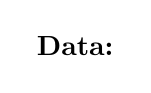
\begin{tikzpicture}[x=1cm,y=0.3cm]
		\node[] (a1) {\textbf{Data:}};			
		\end{tikzpicture}
		}
	\end{minipage}%
	\begin{minipage}{0.35\textwidth}
		\centering
		\subfloat[Dependency among features and prediction]{
			\scalebox{0.4}{	
				\begin{tikzpicture}[x=1.5cm,y=0.3cm]
				% Define nodes
				\node[latent,scale=2] (a1) {$\textrm{age}$} ; %
				\node[obs, scale=2, below=of a1, xshift=-2cm] (h) {$\textrm{fitness}$}; %
				\node[obs, scale=2, below=of a1, xshift=2cm] (i) {$\textrm{income}$}; %
				\node[obs, scale=2, below=of h, xshift=2cm] (p) {$\widehat{Y}$}; %			
				%%add edge
				\edge[] {a1} {h,i} ;
				\edge[] {h,i} {p} ;
				\end{tikzpicture}
			}	
			\label{fairness_fairXplainer_fig:dag_age_income_fitness}}
	\end{minipage}%
	\begin{minipage}{0.4\textwidth}
		\centering
		\subfloat[Age-dependent distributions of non-sensitive features]{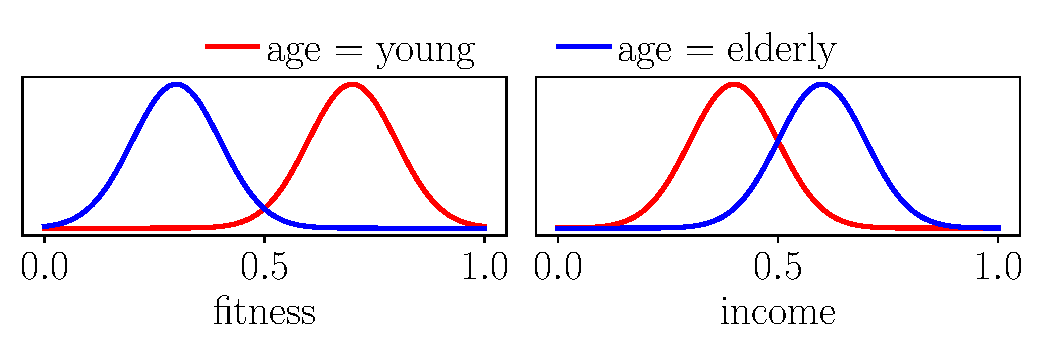
\includegraphics[scale=0.4]{figures/fairness/fif/sanity_distribution}
		\label{fairness_fairXplainer_fig:distribution_example}}
	\end{minipage}

	\begin{minipage}[t]{0.13\textwidth}
		\scalebox{1}{	
			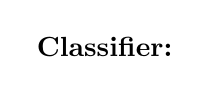
\begin{tikzpicture}[x=1cm,y=0.3cm]
			\node[] (a1) {\textbf{Classifier:}};			
			\end{tikzpicture}
		}
	\end{minipage}%
	\begin{minipage}{0.43\textwidth}
		\centering
		\subfloat[Decision tree (DT$ 1 $)]{
			\scalebox{0.45}{	
				\begin{tikzpicture}[x=1cm,y=1.8cm]
				\node [box, scale=1.5]                                    (p)      {fitness $\geq 0.61$};
				\node [scale=1.5, box, below= of p, xshift=-2.1cm, yshift=1.2cm]    (a1)    {income\\ $\geq 0.29$};
				\node [scale=1.5, box, below= of p, xshift=2.1cm, yshift=1.2cm]     (a2)    {income $\geq 0.69$};
				\node [scale=1.5,below= of a1, xshift=-1.5cm, yshift=0.8cm]  (a11)    { $\widehat{Y}= 1$};
				\node [scale=1.5,below= of a1, xshift=1.5cm, yshift=0.8cm]   (a12)    { $\widehat{Y}=0 $};
				\node [scale=1.5,below= of a2, xshift=-1.5cm, yshift=0.8cm]  (a21)    { $\widehat{Y}= 1$};
				\node [scale=1.5,below= of a2, xshift=1.5cm, yshift=0.8cm]  (a22)    { $\widehat{Y}= 0$};
				%
				\path [line] (p) -|         (a1) node [scale=1.5,midway, above]  {Y};
				\path [line] (p) -|         (a2) node [scale=1.5,midway, above]  {N};
				\path [line] (a1) -|       (a11) node [scale=1.5,midway, above]  {Y};
				\path [line] (a1) -|       (a12) node [scale=1.5,midway, above]  {N};
				\path [line] (a2) -|       (a21) node [scale=1.5,midway, above]  {Y};
				\path [line] (a2) -|       (a22) node [scale=1.5,midway, above]  {N};
				\end{tikzpicture}}
			\label{fairness_fairXplainer_fig:dt_original}}
	\end{minipage}%
	\begin{minipage}{0.45\textwidth}
		\centering
		\subfloat[Decision tree with an affirmative action (DT$ 2 $)]{
			\scalebox{0.45}{	
				\begin{tikzpicture}[x=1cm,y=1.8cm]
				\node [box, scale=1.5]                                    (p)      {fitness $\geq 0.61$};
				\node [scale=1.5, box, below= of p, xshift=-2.1cm, yshift=1.2cm]    (a1)    {income\\ $\geq 0.29$};
				\node [scale=1.5, box, below= of p, xshift=2.1cm, yshift=1.2cm, fill=affirmative]     (a2)    {income $\geq 0.55$};
				\node [scale=1.5,below= of a1, xshift=-1.5cm, yshift=0.8cm]  (a11)    { $\widehat{Y}= 1$};
				\node [scale=1.5,below= of a1, xshift=1.5cm, yshift=0.8cm]   (a12)    { $\widehat{Y}=0 $};
				\node [scale=1.5,below= of a2, xshift=-1.5cm, yshift=0.8cm]  (a21)    { $\widehat{Y}= 1$};
				\node [scale=1.5,below= of a2, xshift=1.5cm, yshift=0.8cm]  (a22)    { $\widehat{Y}= 0$};
				%
				\path [line] (p) -|         (a1) node [scale=1.5,midway, above]  {Y};
				\path [line] (p) -|         (a2) node [scale=1.5,midway, above]  {N};
				\path [line] (a1) -|       (a11) node [scale=1.5,midway, above]  {Y};
				\path [line] (a1) -|       (a12) node [scale=1.5,midway, above]  {N};
				\path [line] (a2) -|       (a21) node [scale=1.5,midway, above]  {Y};
				\path [line] (a2) -|       (a22) node [scale=1.5,midway, above]  {N};
				\end{tikzpicture}}	
			
			\label{fairness_fairXplainer_fig:dt_affirmative}}
	\end{minipage}

	\begin{minipage}[t]{0.07\textwidth}
		%\vspace{-2em}
		\scalebox{1}{	
			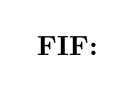
\begin{tikzpicture}[x=1cm,y=0.3cm]
			\node[] (a1) {\textbf{FIF:}};			
			\end{tikzpicture}
		}
	\end{minipage}%
	\begin{minipage}{0.46\textwidth}
		\centering
		\subfloat[Fairness influence functions (FIF) for DT$ 1 $]{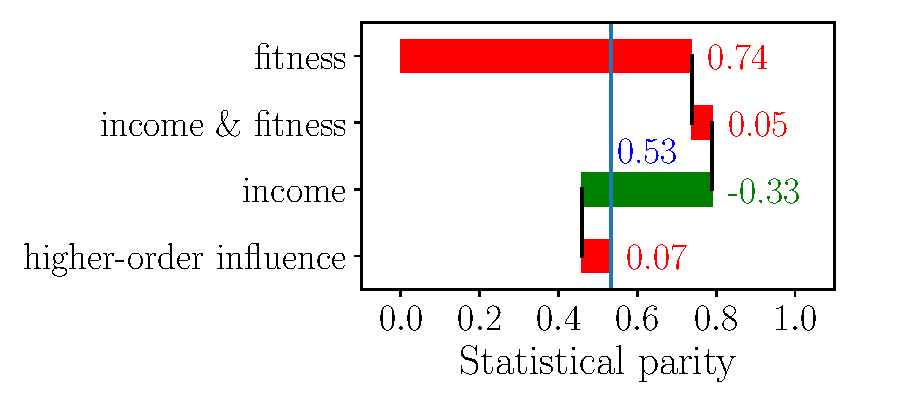
\includegraphics[scale=0.42]{figures/fairness/fif/fif_example}
		\label{fairness_fairXplainer_fig:fif_original}}	
	\end{minipage}%
	\begin{minipage}{0.5\textwidth}
		\centering
		\subfloat[Modified FIFs for DT$ 2 $]{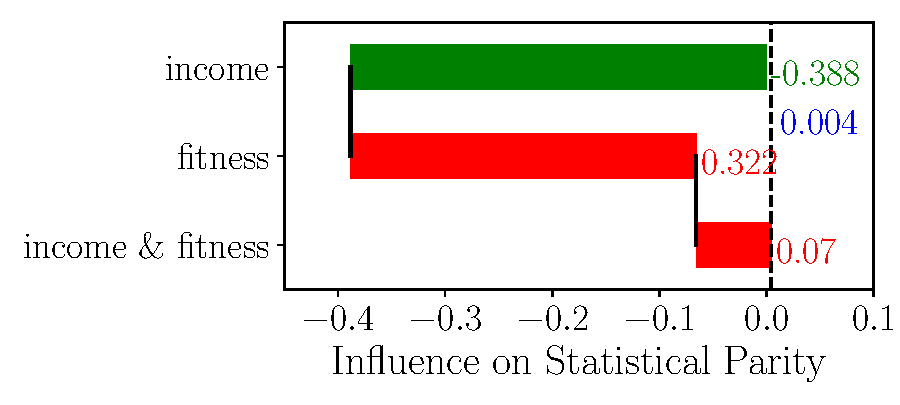
\includegraphics[scale=0.42]{figures/fairness/fif/fif_example_affirmative_action}
		\label{fairness_fairXplainer_fig:fif_affirmative}}
	\end{minipage}
%\vspace*{-.5em}
	\caption[Demonstration of FIF  in health insurance]{FIFs of input features to investigate the bias (statistical parity) of a decision tree predicting the eligibility for health insurance using age-dependent features `fitness' and `income'. An affirmative action reduces bias as corresponding FIFs reflect it.}
	\label{fairness_fairXplainer_fig:fair_example_fif}
	%\vspace{-1.2em}
\end{figure}


\section{Related Work} Recently, several studies apply \emph{local explanation methods} of black-box prediction to explain sources of bias by feature-attribution~\cite{begley2020explainability,lundberg2020explaining} and causal path decomposition~\cite{pan2021explaining}. Since our work adopts feature-attribution approach, it reveals two-fold limitations of existing methods: (i) \emph{inaccuracy} in computing FIFs and (ii) \emph{failing to compute intersectional} FIFs. Elaborately, FIF computation in~\cite{begley2020explainability,lundberg2020explaining} is inaccurate because of applying local explainers such as SHAP~\cite{lundberg2017unified} to compute global properties of the classifier such as group fairness. In addition, features are often correlated in practical fairness tasks, and computing only individual FIFs ignores the joint contribution of multiple features on the unfairness of the classifer. Also, these works provide empirical evaluations to justify the choices of SHAP-based tools for explaining fairness and does not consider the global nature of group fairness metrics. In this chapter, \textit{we develop a formal framework to explain sources of unfairness in a classifier and also a novel methodology to address it. To the best of our knowledge, this is the first work to do the both}. %\todo{1. GSA with fairness, 2. Citation not correct, 3. Influence of Yair Zick.}
Among other related works, \cite{benesse2021fairness} link GSA measures such as Sobol and Cram{\'e}r-von-Mises indices to different fairness metrics. While their approach relates the GSA of sensitive features on the resulting bias, we focus on applying GSA to all features to compute FIFs. \textit{Their approach only detects the presence or absence of bias, while we focus on decomposing bias as the sum of FIFs of all features}. In another line of work, \cite{datta2016algorithmic} and \cite{ghosh2022algorithmic} compute feature-influence as the shift of bias from its original value by randomly intervening features. Their work is different from our axiomatic approach, where the sum of FIFs equals the bias.
